\chapter{研究動機}
\section{應用環境}
\begin{figure}[!htbp]
\centering
\scalebox{.35}{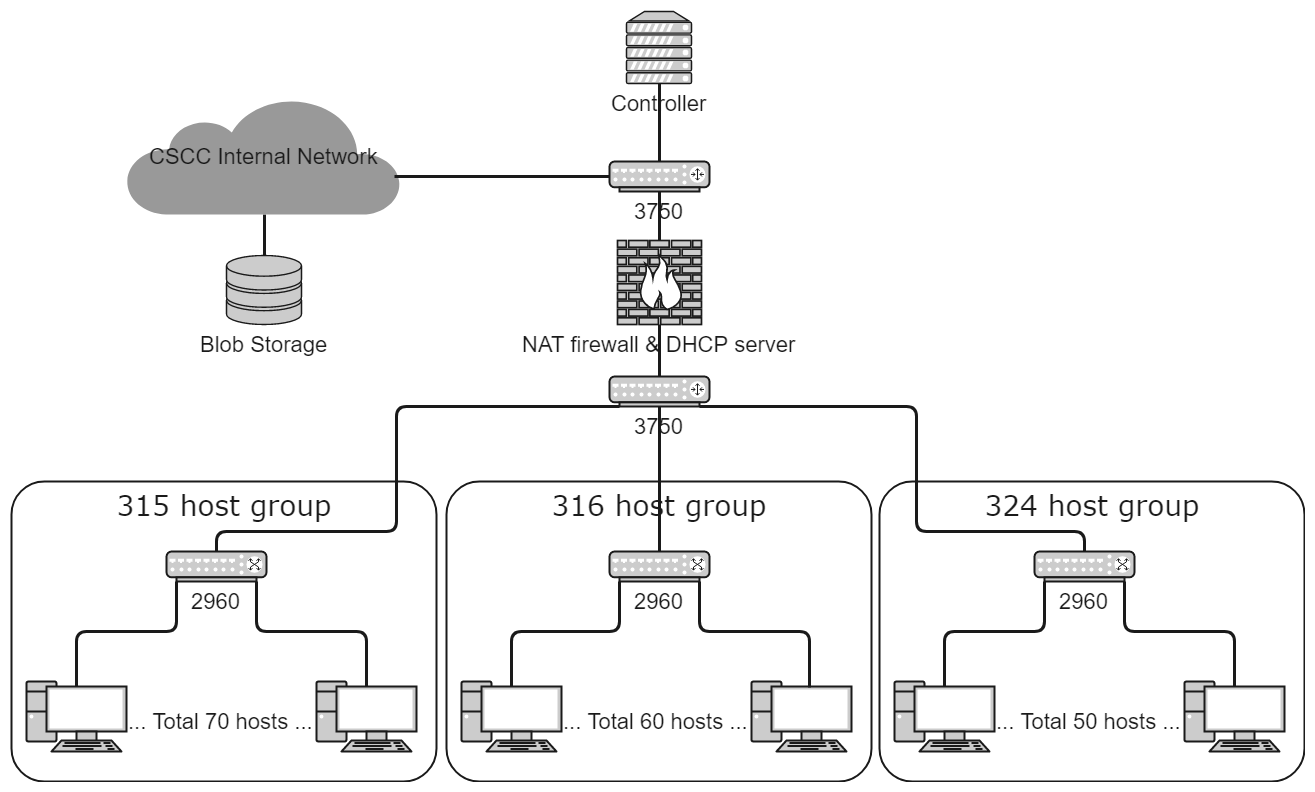
\includegraphics{images/PC_Room_Network.png}}
\caption{PC Room Network.}
\label{i:pcroom}
\end{figure}



在交通大學資訊工程學系計算機中心,需要大量部署 PC 電腦教室 Windows 作業系統與管理。
從圖 \ref{i:pcroom} 可以看見計算機中心有三個主機群,主機數量分別為 50 台在 324 主機群、60 台在 316 主機群、70 台在 315 主機群,總共有 180 台主機需要部署作業系統與組態管理。
每學期都必須重新安裝作業系統以及更新課程軟體,準備單台機器的時間超過一天以上,並且難以將安裝過程自動化。
因此我們會準備一台原型機,將其系統製作成映像檔,部署到其他主機上。


以部署系上課程用的映像檔為例,映像檔大小約為 100 GB,若使用三台部署伺服器,各伺服器的硬碟連續讀取速率約為 200 MB/s ,透過一對一的方式傳輸映像檔到所有主機群共 180 台主機,在最佳情況下所需要花費的時間為 512 分鐘。然而一般情況需要考量硬碟隨機讀取速度,且若減少部署伺服器到一台所需時間將倍增為 1536 分鐘,不可能應用在大規模的計算中心。
原先期望透過基於 Multicast 技術的 Clonezilla Server Edition 加速部署作業,然而其在部署速度和穩定度皆不盡理想。

\section{裸機再生}
每門課程的使用需求不盡相同,需要不同的應用程式或虛擬機器,因此一台主機中會包含上萬個檔案且佔用數百 GB 的硬碟空間。若採用檔案層級再生(file-level cloning)的映像檔,必須仰賴作業系統與檔案系統,不僅會影響部屬效率,也無法確保部屬後實體主機的一致性,可能會導致檔案毀損或遺失等情況。
區塊層級再生(block-level cloning)則是完整複製硬碟區塊,由於是讀寫連續的區塊,在部署上有一定的效率,也能完整複製原型機的硬碟區塊到目標主機上。
本研究認為區塊層級再生(block-level cloning)的映像檔在裸機服務開通系統上是重要的功能,我們可以透過區塊層級再生確保映像檔與實體主機的一致性與完整性,因此在開發 BitFission 上採用區塊層級再生來製作映像檔。
\section{映像檔部屬}
以往在電腦教室中,我們透過最普遍的多播傳輸部屬映像檔到各台主機上。
但是多播傳輸必須確保每一台主機在部屬進度上的一致性,如果發生單台主機失去回應(unresponsive)便會阻塞多播傳輸。
尤其在頻繁使用的電腦教室中,硬體老化提高了單台主機故障的機率,大幅降低了多播傳輸的效率。
此外,即使沒有主機故障或是失去回應,仍有許多因素會造成多播傳輸的速度下滑,例如單台主機的硬碟寫入延遲。
一般而言,我們需要耗費相當的人力去偵錯,因為多播傳輸的一致性,讓熱點(hotspots)難以被判別。
因此在裸機服務開通上,本研究認為需要有更加快速且更可靠的傳輸方法,解決上述各項部屬的問題。
\section{組態設定}
基於課程需求,我們大多數的映像檔是使用 Windows 作業系統,但並不受限於之。
即便可以透過 Windows AD 或是 winrm 等技術遠端進行組態設定,在多台主機上進行狀態控制與例外處理仍需要人工作業。
本研究期望有一個無人值守的組態設定流程以及即時的狀況監控,如今許多跨平台的開源組態管理工具可以達到上述的需求。
因此本研究分析了一些組態設定工具,決定何者適合做為 BitFission 的組態管理系統核心工具。

\section{研究目標}
綜合以上所有動機,本研究有以下目標:
\begin{enumerate}
\item 區塊層級再生的映像檔
\item 容錯無回應主機的傳輸機制
\item 可規模化的映像檔部署方法
\item 無人值守的部署流程
\item 基於開放原始碼專案的裸機服務開通框架
\end{enumerate}

